\documentclass[b5paper]{ctexrep}
\usepackage[margin=1in]{geometry}
% This preamble is heavily inspired by Soham Chatterjee's work in
% https://github.com/sohamch08/Eye-Candy-Lecture-Notes-Theme

% tex-fmt: off
% cSpell: disable
%%%%%%%%%%%%%%%%%%%%%%%%%%%%%%%%%
% PACKAGE IMPORTS
%%%%%%%%%%%%%%%%%%%%%%%%%%%%%%%%%

\usepackage{amsthm}
\usepackage{amsmath}
\usepackage{amssymb}
\usepackage{booktabs}  % 提供更专业的表格线条
% Provide support for minipage used in definition environment
\usepackage{varwidth}
\usepackage[backend=biber,style=authortitle]{biblatex}
\usepackage{array}     % 增强的表格功能
% Underline and strikethrough
\usepackage[normalem]{ulem}
\usepackage[dvipsnames]{xcolor}
\usepackage[most,many,breakable]{tcolorbox}
\usepackage{extarrows}
\usepackage{derivative}
\usepackage{tikz-cd}
% Make sure all math formulas are displayed in displaystyle
\usepackage{breqn}
% Some may argue that the use of displaystyle in inline formulas may
% break line spacing and make the document look ugly. However, I
% prefer to follow the choice of the textbook setting
\everymath{\displaystyle}
% For \mathscr
\usepackage{mathrsfs}
\usepackage{graphicx}
% Title and ToC format
\usepackage{titletoc,titlesec}
\usepackage{float}
\usepackage{tikz}
% For bold math symbols
\usepackage{bm}
\usepackage{mathtools} % For \coloneqq
\usepackage{hyperref}
\hypersetup{%
 colorlinks=true, linkcolor=mydoccolor!80, urlcolor=mydoccolor!80,
 citecolor=mycitecolor!80!black,
 bookmarksnumbered=true,
 bookmarksopen=true
}
\usepackage{cleveref}
% Use verb inside other environments
\usepackage{fancyvrb}
\VerbatimFootnotes
\SaveVerb{smile}|:-)|
\SaveVerb{laugh}|:-D|
\SaveVerb{wink}|;-)|
\SaveVerb{sad}|:-(|
\SaveVerb{angry}|:-@|
\SaveVerb{confused}|:-S|
\SaveVerb{cool}|B-)|
\SaveVerb{cry}|:'-|
\SaveVerb{kiss}|:-*|
\SaveVerb{surprised}|:-o|
\SaveVerb{grin}|:-]|
\SaveVerb{naughty}|:P|
% \setCJKmainfont[BoldFont=SimHei,ItalicFont=FangSong,BoldItalicFont=LiSu]{SimSun}
% For cancel line
\usepackage{cancel}
% For code highlighting
\usepackage{listings}
\newfontfamily{\Cascadia}{Cascadia Code}
\lstset{language=Mathematica}
\lstset{basicstyle={\Cascadia\footnotesize},
    numbers=left,
    numberstyle=\tiny\color{gray},
    numbersep=5pt,
    breaklines=true,
    captionpos={t},
    frame={lines},
    rulecolor=\color{black},
    framerule=0.5pt,
    columns=flexible,
    tabsize=4
}
%%%%%%%%%%%%%%%%%%%%%%%%%%%%
% Custom commands
%%%%%%%%%%%%%%%%%%%%%%%%%%%%

%================================
% PAGE SETUP
%================================

\renewcommand{\thesection}{\textbf{\chinese{section}}、\hspace{-1em}}
\renewcommand{\thesubsection}{\arabic{subsection}.\hspace{-0.3em}}
\renewcommand{\thesubsubsection}{\arabic{subsubsection}}
\catcode`\。=\active\newcommand{。}{.}
\ctexset{section={format={\Large\raggedright\bfseries}}}
%================================
% MATH COMMANDS
%==========================\hl{}===
\AtBeginDocument{%
\renewcommand\Re{\operatorname{Re}}
\renewcommand\Im{\operatorname{Im}}
}
\renewcommand{\i}{\mathrm{i}}
\newcommand{\e}{\mathrm{e}}
\renewcommand{\d}{\odif}

\newcommand{\R}{\mathbb{R}} % Real
\newcommand{\C}{\mathbb{C}} % Complex
\newcommand{\Z}{\mathbb{Z}} % Integer, from Zahlen, by David Hilbert
\newcommand{\Q}{\mathbb{Q}} % Rational, from Quotient
\newcommand{\N}{\mathbb{N}} % Natural, from Naturals

\newcommand{\abs}[1]{\left|#1\right|} % Absolute value

\newcommand{\placeholder}[1]{\mathrel{\phantom{#1}}} % Placeholder

\crefname{equation}{式}{式}
\Crefname{equation}{式}{式}
\crefname{theorem}{定理}{定理}
\Crefname{theorem}{定理}{定理}
\crefname{definition}{定义}{定义}
\Crefname{definition}{定义}{定义}
\crefname{problem}{问题}{问题}
\Crefname{problem}{问题}{问题}
\crefname{claim}{断言}{断言}
\Crefname{claim}{断言}{断言}
\crefname{note}{注}{注}
\Crefname{note}{注}{注}

%================================
% DOCUMENT SETUP
%================================

\newcommand\hl{\bgroup\markoverwith{\textcolor{yellow}{\rule[-.5ex]{2pt}{2.5ex}}}\ULon}

\newfontfamily\DancingScript{Dancing Script OT}
\newcommand{\Caffein}{\DancingScript{Caffein3}}

%%%%%%%%%%%%%%%%%%%%%%%%%%%%%%
% COLORS
%%%%%%%%%%%%%%%%%%%%%%%%%%%%%%
\definecolor{myclaimcolor}{RGB}{56, 140, 70}
\definecolor{mynoteolor}{RGB}{56, 140, 70}
\definecolor{mytheoremcolor}{RGB}{0,102,204}
\definecolor{mydefinitioncolor}{RGB}{235, 105,12}
\definecolor{myquotecolor}{RGB}{161,143,125}
\definecolor{mycitecolor}{RGB}{0, 102, 204}
\definecolor{myproblemcolor}{RGB}{255,128,0}
\definecolor{mydoccolor}{RGB}{141,64,13}

%%%%%%%%%%%%%%%%%%%%%%%%%%%%%%%%%%%%%%%%%%%
% TABLE OF CONTENTS
%%%%%%%%%%%%%%%%%%%%%%%%%%%%%%%%%%%%%%%%%%%

% Let's just hope I won't use chapter more than 10 times
\usetikzlibrary{shapes, positioning}
\contentsmargin{0cm}
\titlecontents{chapter}[3.7pc]
{\addvspace{30pt}%
    \begin{tikzpicture}[remember picture, overlay]%
        \draw[fill=mydoccolor!60,draw=mydoccolor!60]
        (-7,-.1) rectangle (-0.6,.5);%
        \pgftext[left,x=-2.5cm,y=0.2cm]{\color{white}\Large\bfseries
        \thecontentslabel};%
\end{tikzpicture}\color{mydoccolor!60}\large\bfseries}%
{}
{}
{\;\titlerule\;\large\bfseries Page \thecontentspage
    \begin{tikzpicture}[remember picture, overlay]
        \draw[fill=mydoccolor!60,draw=mydoccolor!60]
        (2pt,0) rectangle (4,0.1pt);
\end{tikzpicture}}%
\titlecontents{section}[3.7pc]
{\addvspace{2pt}}
{\contentslabel[\textcolor{mydoccolor!80}\thecontentslabel]{2pc}}
{}
{\hfill\small \thecontentspage}
[]
\titlecontents{subsection}[2.7pc]
{\addvspace{-1pt}\small}
{\hspace*{2pc}\contentslabel[\textcolor{mydoccolor!80}\thecontentslabel]{1pc}}
{}
{\hfill\small \thecontentspage}
[]

%{\addvspace{-1pt}\small}
%{}
%{}
%{\ --- \small\thecontentspage}
%[ \textbullet\ ][]

\makeatletter
\renewcommand{\tableofcontents}{%
    \chapter*{%
        \vspace*{-80\p@}%
        \begin{tikzpicture}[remember picture, overlay]%
            \pgftext[right,x=15cm,y=0.2cm]{\color{mydoccolor!60}\Huge\bfseries
            \contentsname};%
            \draw[fill=mydoccolor!60,draw=mydoccolor!60] (13,-.75)
            rectangle (20,1);%
            \clip (13,-.75) rectangle (20,1);
            \pgftext[right,x=15cm,y=0.2cm]{\color{white}\Huge\bfseries
            \contentsname};%
    \end{tikzpicture}}%
\@starttoc{toc}}
\makeatother
%\titleformat{\chapter}[display]
%{\normalfont\Huge\bfseries}{\chaptertitlename\ \thechapter}{20pt}{\Huge}

\newcommand\colorlink[3]{\href{#2}{\color{#1}#3}}
\newcommand\colorurl[2]{{\color{#1}\url{#2}}}

%%%%%%%%%%%%%%%%%%%%%%%%%%%%
% New environments
%%%%%%%%%%%%%%%%%%%%%%%%%%%%
%! Caution: All environments with CAPITALIZED first letter
%! is for internal use only
\tcbuselibrary{theorems,skins,hooks}
%================================
% THEOREM BOX
%================================
\makeatletter
\newtcbtheorem[number within=chapter]{Theorem}{Theorem}{enhanced,
    breakable,
    colback=mytheoremcolor!8,
    colframe=mytheoremcolor,
    attach boxed title to top left={yshift*=-\tcboxedtitleheight},
    fonttitle=\bfseries,
    title={#2},
    boxed title size=title,
    boxed title style={%
        sharp corners,
        rounded corners=northwest,
        colback=tcbcolframe,
        boxrule=0pt,
    },
    underlay boxed title={%
        \path[fill=tcbcolframe] (title.south west)--(title.south east)
        to[out=0, in=180] ([xshift=5mm]title.east)--
        (title.center-|frame.east)
        [rounded corners=\kvtcb@arc] |-
        (frame.north) -| cycle;
    },
    #1
}{theorem}
\makeatother

\newenvironment{theorem}[2][]{%
    \begin{Theorem}{#2}{#1}%
    }{%
    \end{Theorem}%
}

%================================
% DEFINITION BOX
%================================
\makeatletter
\newtcbtheorem[number
within=chapter]{Definition}{Definition}{enhanced,
    breakable,
    colback=mydefinitioncolor!8,
    colframe=mydefinitioncolor,
    attach boxed title to top left={yshift*=-\tcboxedtitleheight},
    fonttitle=\bfseries,
    title={#2},
    boxed title size=title,
    boxed title style={%
        sharp corners,
        rounded corners=northwest,
        colback=tcbcolframe,
        boxrule=0pt,
    },
    underlay boxed title={%
        \path[fill=tcbcolframe] (title.south west)--(title.south east)
        to[out=0, in=180] ([xshift=5mm]title.east)--
        (title.center-|frame.east)
        [rounded corners=\kvtcb@arc] |-
        (frame.north) -| cycle;
    },
    #1
}{definition}
\makeatother

\newenvironment{definition}[2][]{%
    \begin{Definition}{#2}{#1}%
    }{%
    \end{Definition}%
}

%================================
% PROBLEM BOX
%================================
\newtcbtheorem[number within=chapter]{Problem}{Problem}
{%
    enhanced,
    breakable,
    colback = myproblemcolor!10,
    frame hidden,
    boxrule = 0sp,
    borderline west = {2pt}{0pt}{myproblemcolor},
    sharp corners,
    detach title,
    before upper = \tcbtitle\par\smallskip,
    coltitle = myproblemcolor!85!black,
    fonttitle = \bfseries\sffamily,
    description font = \mdseries,
    separator sign none,
    segmentation style={solid, myproblemcolor!85!black},
}
{problem}

\newenvironment{problem}[2][]{%
    \begin{Problem}{#2}{#1}%
    }{%
    \end{Problem}%
}
%================================
% CLAIM BOX
%================================
\newtcbtheorem[number within=chapter]{Claim}{Claim}
{%
    enhanced
    ,breakable
    ,colback = myclaimcolor!10
    ,frame hidden
    ,boxrule = 0sp
    ,borderline west = {2pt}{0pt}{myclaimcolor}
    ,sharp corners
    ,detach title
    ,before upper = \tcbtitle\par\smallskip
    ,coltitle = myclaimcolor!85!black
    ,fonttitle = \bfseries\sffamily
    ,description font = \mdseries
    ,separator sign none
    ,segmentation style={solid, myclaimcolor!85!black}
}
{claim}

\newenvironment{claim}[2][]{%
    \begin{Claim}{#2}{#1}%
    }{%
    \end{Claim}%
}

%================================
% NOTE BOX
%================================

\newtcbtheorem[number within=chapter]{Note}{Note}
{%
    enhanced
    ,breakable
    ,colback = mynotecolor!10
    ,frame hidden
    ,boxrule = 0sp
    ,borderline west = {2pt}{0pt}{mynotecolor}
    ,sharp corners
    ,detach title
    ,before upper = \tcbtitle\par\smallskip
    ,coltitle = mynotecolor!85!black
    ,fonttitle = \bfseries\sffamily
    ,description font = \mdseries
    ,separator sign none
    ,segmentation style={solid, mynotecolor!85!black}
}
{note}

\newenvironment{note}[2][]{%
    \begin{Note}{#2}{#1}%
    }{%
    \end{Note}%
}
%================================
% QUOTE BOX
%================================
\newtcolorbox{refbox}[1][]{%
enhanced,
breakable,
colback = myquotecolor!10,
frame hidden,
boxrule = 0sp,
borderline west = {2pt}{0pt}{myquotecolor},
sharp corners,
#1
}
\renewenvironment{quote}{%
\begin{refbox}}{%
\end{refbox}}
% Extra Information
% INFO: Use \mathclap and \substack to create multiline

\begin{document}
\title{概率论笔记}
\author{\Large \Caffein}
\date{}
\maketitle
\tableofcontents

% Define a custom command for probability notation
\renewcommand{\P}[1]{P\left\{#1\right\}}

% Laplace transform
\renewcommand{\L}[1]{\mathcal{L}\left\{#1\right\}}
% Inverse Laplace transform
\newcommand{\invL}[1]{\mathcal{L}^{-1}\left\{#1\right\}}
% % !TeX root = main.tex
\chapter*{写在前面}
% TODO: Change the tone of the preface to be more humorous
% and engaging.
大部分中国的线性代数教材, 开篇多以逆序数从天而降的给出行列式的定义
% TODO: Why it involves permutation? See 3b1b's video
% on determinants
(殊不知行列式逆序数概念的定义本身就需要用到抽象代数\(S_{n}\) 的知识), 偌大的代数体系建立于行列式之上,
学生们上来就陷入行列式技巧计算的泥潭, 课本大量有用的知识还深藏在无头习题里(没有出处与附注的关键习题).
教材含糊其辞,学生雾里看花,最终一个学期下来,
学生们对线性代数的理解仅仅停留在机械计算上, 对着抽象的代数概念望洋兴叹, 感叹大学数学的``厉害''.

这是笔者第二次学习线性代数. 选用的教材是大名鼎鼎的 \emph{Linear Algebra Done
Right}.
相较于国内大部分数学教材, 这本书不以集合论开头, 不以抽象的行列式概念导入,
在能补充的部分都有详尽的补充(生怕我看不明白). 希望能借以此书, 加深自己对线性代数的理解.

% % !TeX root = main.tex

\chapter{Gamma 函数与Beta 函数}

\section{Gamma 函数}
\[
    \Gamma(x) = \int_0^\infty t^{x-1} e^{-t} dt
\]
\[
    \Gamma(n) = (n-1)\Gamma(n-1)
\]
\[
    \Gamma^{(n)}(x) = \int_0^\infty t^{x-1} e^{-t} \ln^n t \, dt
\]
倍元公式
\[
    \Gamma(2s) = 2^{2s-1} \sqrt{\pi}
    \frac{\Gamma(s)}{\Gamma(s+\frac{1}{2})}
\]
余元公式
\[
    \betafunc(s, 1-s) = \frac{\pi}{\sin(\pi s)} = \Gamma(s)
    \Gamma(1-s)
\]
\section{Beta 函数}

\[
    \betafunc(x, y) = \int_0^1 t^{x-1} (1-t)^{y-1} dt
\]
\[
    \betafunc(x, y) = \frac{\Gamma(x) \Gamma(y)}{\Gamma(x+y)}
\]
(化圆为方)
\[
    \betafunc(p ,q+1) = \frac{q}{p+q} \betafunc(p,q) \quad
    \betafunc(p+1, q) = \frac{p}{p+q} \betafunc(p,q)
\]
(递推求解)
\subsection{可求解的积分}
\[
    \int_{0}^{+\infty} x^{a-1} \e^{-x^{b}} \d{x} =
    \frac{1}{a} \Gamma\left( \frac{a}{b} +1 \right) = \frac{1}{b}
    \Gamma\left(\frac{a}{b}\right)
\]
\[
    \int_{0}^{\frac{\pi}{2}} \sin^{m} x \cos^{n} x \d{x} =
    \frac{1}{2} \betafunc\left(\frac{m+1}{2}, \frac{n+1}{2}\right)
\]
\[
    \int_{0}^{\infty} \sinh^{m} x \cosh^{n} x \d{x} =
    \frac{1}{2} \betafunc\left(\frac{m+1}{2}, -\frac{m+n}{2}\right)
\]
\[
    \int_{0}^{+\infty } \frac{x^{p-1}}{(1+x)^{p+q}} \d{x} =
    \betafunc(p, q)
\]
% TODO: 用\(t/t+1\)对beta函数进行变换
% TODO: 用t^alpha对beta函数进行变换
% % !TeX root = main.tex
\chapter{平面几何}

\section{什么是共轭}

在抽象代数中我们接触过很多代数结构里的抽象概念,诸如正规化子,交换子,中心等等等等。
其中最先出现也最先困惑我们的就是\emph{共轭}这个概念。

\section{一个例子}
考虑Euclid平面的保距变换群(这个名词是什么并不重要)。\(g\) 表示是绕原点\(O\)
旋转\(\theta\degree\) 的旋转变换。\(h\) 表示沿向量\(v\) 的平移变换,
并把原点\(O\) 移动到点\(A\)。那么我们如何表示绕点\(A\) 旋转\(\theta\degree\)
的变换呢?很简单,先把\(A\) 点移动到\(O\) 点(对平面上的点做变换\(h^{-1}\)),
再做绕原点的旋转变换\(g\),最后再将原点平移至点\(A\) (做变换\(h\)),也就是做复合变换\(hgh^{-1}\)。
% TODO: Fix this
\begin{figure}[ht]
    \centering
    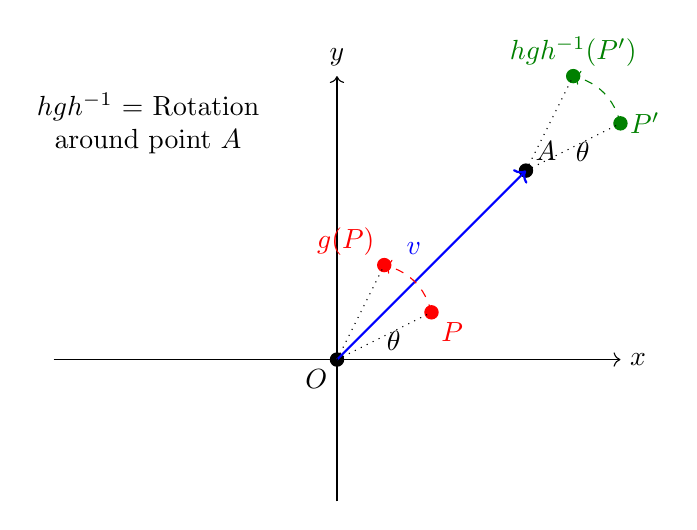
\begin{tikzpicture}[scale=1.2]
        % Coordinate system
        \draw[->] (-3,0) -- (3,0) node[right] {$x$};
        \draw[->] (0,-1.5) -- (0,3) node[above] {$y$};

        % Original point O and point A
        \filldraw[black] (0,0) circle (2pt) node[below left] {$O$};
        \filldraw[black] (2,2) circle (2pt) node[above right] {$A$};

        % Translation vector
        \draw[->, thick, blue] (0,0) -- (2,2) node[midway,
        above left] {$v$};

        % Point P and its image under rotation around O
        \filldraw[red] (1,0.5) circle (2pt) node[below right] {$P$};
        \filldraw[red] (0.5,1) circle (2pt) node[above
        left] {$g(P)$};
        \draw[->, dashed, red] (1,0.5) to[bend right] (0.5,1);
        \draw[dotted] (0,0) -- (1,0.5);
        \draw[dotted] (0,0) -- (0.5,1);
        \node at (0.6,0.2) {$\theta$};

        % Point P' = h(P) and its image under rotation around A
        \filldraw[green!50!black] (3,2.5) circle (2pt)
        node[right] {$P'$};
        \filldraw[green!50!black] (2.5,3) circle (2pt)
        node[above] {$hgh^{-1}(P')$};
        \draw[->, dashed, green!50!black] (3,2.5) to[bend
        right] (2.5,3);
        \draw[dotted] (2,2) -- (3,2.5);
        \draw[dotted] (2,2) -- (2.5,3);
        \node at (2.6,2.2) {$\theta$};

        % Explanation labels for conjugation
        \node[align=center] at (-2,2.5) {$hgh^{-1}$ =
        Rotation\\around point $A$};
    \end{tikzpicture}
    \caption{共轭变换 $hgh^{-1}$ 表示绕点 $A$ 旋转 $\theta$ 度}
\end{figure}

瞧,这正是共轭的定义。

\section{什么是共轭}

\begin{quotation}
    One way to think about conjugation is as a
    generalization of changing coordinates when rewriting
    matrices or, from a physical point of view, as the
    process of "seeing a group from a different perspective."

    In other words, what conjugation does in terms of group
    actions (and it is always a good idea to think of groups in
    terms of their actions) is it corresponds to a "change of
    coordinates" on the underlying set \(X\)
    . This is a basic reason conjugation and group theory are
    important in understanding Newtonian mechanics (where \(G\)
    is the Galilean group) or relativity (where \(G\)
    is the Lorentz group) or really much of modern physics in
    general: in physics groups are always studied because of
    their actions and we always want our concepts and equations
    to be invariant under these actions. (For example, mass and
        charge are invariant concepts. The mass or charge of an
    object doesn't change when you rotate or translate it.)

    This gives a very intuitive definition of a normal
    subgroup: it's a subgroup that "looks the same from every
    perspective." For example, the subgroup of translations in
    the Euclidean group is always normal because the
    description "\(g\)
    is a translation" is the same from every perspective (that
    is, it's invariant under conjugation). It's a good exercise
    to look at some groups you're familiar with and see if you
    can identify which subgroups are normal based on this
    principle. (This principle underlies the importance of
    normal subgroups in Galois theory as well.)
\end{quotation}

从我个人的理解来看,共轭起``重命名''的作用,具有换基的功能。
它可以把原先作用在原点处的东西转化为在别处的作用,从而让别的地方``旋转''成为了可能。

\section{为什么共轭如此神奇}
读完以上内容不免心生疑惑,为什么共轭如此神奇?为什么一个简单的\(hgh^{-1}\) 组合就能实现换基?
就以刚刚的例子为例,为什么平移变换复合过后旋转中心就变到了\(A\) 点?难道在复合的过程中旋转不会变形吗?

这个问题其实可以拆成两个部分:
\subsection{为什么在复合的过程中旋转不会变形?}
什么是变形?

事实上,我们考虑全体以原点为中心的旋转构成的子群。我们不难发现把旋转转换到\(A\) 点的\(hgh^{-1}\)
已经并不属于这个子群。在这个意义上,这个变换已经变形了。

如果``不变形''指的是变换过后的旋转依然是一个旋转,实际上平面上全体旋转构成的集合压根不构成一个群。

\subsection{为什么 \(hgh^{-1}\) 组合能实现换基?}

\href{https://math.stackexchange.com/questions/11971/intuition-behind-conjugation-in-group-theory}{讨论}

% !TeX root = main.tex
\chapter{等距变换群\(\Isom \R^{2}\)}
% Chapter1: 旋转与狄利克雷逼近和. . . 逼近

\section{Basics}

\subsection{为什么结合律如此重要?}
我们早已熟悉结合律和交换律,并能轻松的找出满足其一而不满足其二的二元运算\footnote{其实参考了
    \href{https://math.stackexchange.com/questions/608280/real-life-examples-of-commutative-but-non-associative-operations}{Stack
    Exchange}
讨论\UseVerb{naughty}}:

\begin{description}
    \item[满足交换律而不满足结合律:] \(a \otimes b \coloneqq \frac{a+b}{2}\)
    \item[满足结合律而不满足交换律:] 矩阵乘法
\end{description}

交换律和结合律看起来同样的重要,可为什么我们选择了结合律作为群的定义而不是交换律呢?

答案很简单,群最初是研究对称的学问。而对称的复合,正如函数的复合,满足结合律而不一定满足交换律。
那为什么函数的复合满足结合律呢?

\begin{theorem}{函数的复合满足结合律}
    设\(f: X\to Y\),\(g: Y\to Z\),\(h: Z\to W\)是任意函数,则
    \[
        h\circ(g\circ f)=(h\circ g)\circ f
    \]
\end{theorem}

\begin{proof}
    \(\forall x\in X\),则
    \begin{align*}
        [h\circ(g\circ f)](x) & = h(g \circ f(x))  & = h(g(f(x))) \\
        [(h\circ g)\circ f](x) & = (h\circ g)(f(x)) & = h(g(f(x)))
    \end{align*}
\end{proof}

\begin{quote}
    Young man, in mathematics you don't understand things.
    You just get used to them.

    \hfill ---John von Neumann
\end{quote}

编程过多的同学看到这里可能会疑惑,世间那么多事物都可以抽象成纯函数,函数的复合居然满足结合律,
这背后一定有着更深刻的道理\footnote{其实我们困惑主要在其反直觉性:结合律居然对广泛的函数运算都成立。
    实际上这个定理并没有那么强。这里的二元运算已被规定为函数复合,该定理只告诉我们对于输出严格确定唯一输入的纯函数,
应用时间与结果无关。在现实生活中可以理解为三个模块按顺序叠加并不影响其功能}

一个函数\(f: X \to Y\)实际上可以看作集合\(X \times Y\) 上的一个子集\(F\)。
\begin{definition}{函数(的像)}
    称\(f: X\to Y\) 是一个函数,如果:

    对于任意\(x\in X\),存在唯一的\(y\in Y\)使得二元关系\(x \circ_{f} y\)
    成立,即\((x,y)\in F\)
\end{definition}

两个函数相等实际上就是对于相同的自变量\(x\)对应相同的值\(y\)。
而函数的复合就可以定义为:
\begin{definition}{函数的复合}
    设\(f: X\to Y\),\(g: Y\to Z\),则\(g\circ f: X \to Z\)是一个函数,使得
    \[
        x \circ_{g\circ f} z \iff \exists! y \in Y, x
        \circ_{f} y \land y \circ_{g} z
    \]
    其中\(x\in X\),\(y\in Y\),\(z\in Z\)。
    \end{definition}
    有了以上的定义我们就能够用量词更确切的告诉我们函数的复合性是成立的。
\begin{proof}
    \(\forall x \in X\):
    \begin{align*}
        &\mathrel{\phantom{\iff}}w=h \circ(g\circ f)(x) \\
        &\iff \exists! z \in Z, x \circ_{f\circ g} z \land z
        \circ_{h} w\\
        &\iff \exists! z \in Z, \exists! y \in Y, x
        \circ_{f} y \land y \circ_{g} z \land z
        \circ_{h} w\\
    \end{align*}
    而:
    \begin{align*}
        &\mathrel{\phantom{\iff}}w=(h\circ g)\circ f(x) \\
        &\iff \exists! y \in Y, x \circ_{f} y \land y
        \circ_{g \circ h} w\\
        &\iff \exists! y \in Y, \exists! z \in Z, x
        \circ_{f} y \land y
        \circ_{g} z \land w
    \end{align*}
\end{proof}

\subsection{交换图}

\begin{definition}
    一个交换图是一个图,其中所有具有相同起点和终点的有向路径都导致相同的结果。
    \begin{figure}[H]
        \centering
        \begin{tikzcd}
            G_{1} \times G_{1} \arrow[rr, "*_{1}"] \arrow[d,
            "{(\varphi,\varphi)}"] &  & G_{1} \arrow[d, "\varphi"] \\
            G_{2} \times G_{2} \arrow[rr, "*_{2}"]
            &  & G_{2}
        \end{tikzcd}
        \caption{一个交换图的例子}
    \end{figure}
\end{definition}

\section{等距变换群与半直积}

\begin{quote}
    希腊语单词 isos 意为相等、metron 意为度量,所以 isometry 的字面意思就是度量相等。
    \hfill ---\textit{Linear Algebra Done Right}
\end{quote}

\begin{definition}{半直积}
    给定任意两个群\(N\)和\(H\)以及群同态\(\phi: H \to \Aut{N}\),我们在集合\(H
    \times N\) 上定义二元运算\(\circ\):
    \begin{align*}
        \circ : (H\times N)\times (H\times N) & \to H\times N \\
        ((h_{1}, n_{1}), (h_{2}, n_{2})) & \mapsto
        (h_{1}h_{2}, \phi(h_{1})(n_{2})n_{1})
    \end{align*}
    则\((H\times N, \circ )\) 构成一个群,称为\(H\)和\(N\)的半直积,
    记作\(H\ltimes N\)
\end{definition}

半直积是广泛存在的结构
% TODO: 半直积的几何意义
\begin{enumerate}
    \item \(D_{2n}\cong C_{2}\ltimes C_{n}\) (注意到\(\Aut
        C_{n}\cong U_{n}\)),其中
        \begin{align*}
            \phi: C_{2} & \to \Aut{C_{n}} \\
            b^{k} & \mapsto
            \begin{cases}
                f(a)  = a, & k=0 \\
                f(a)  = a^{-1}, &k=1
            \end{cases}
        \end{align*}
    \item \(O(n)\cong C_{2} \ltimes SO(n)\)
        % TODO: How to prove this?
\end{enumerate}

于是我们可以验证
\[
    \Isom \R^{2} \cong O(2) \ltimes \R^{2}
\]
半直积形状为何如此
半直积的几何意义

\section{\(\Isom \R^{2}\) 的一些子群}
\begin{enumerate}
    \item \(\langle R_{\theta} \rangle\cong \Z\)
    \item \(\langle T_{\theta} \rangle\cong \Z\)
    \item \(\langle T_{a,b} \rangle\cong \Z^{2}\)(\(a\),\(b\) 线性无关)
\end{enumerate}

\section{群作用}
New notations, new toys!

抽象代数里曾指出所有群都同构于置换群的一个子群,也就是\textit{群作用}:

\begin{definition}{群作用}
    设\(G\)是一个群,\(X\)是一个集合,\(G\)在\(X\)上的作用是一个映射
    \begin{align*}
        \Phi: G\times X & \to X \\
        (g,x) & \mapsto g\cdot x
    \end{align*}
    使得对于任意\(g,h\in G\),\(x\in X\),都有
    \begin{enumerate}
        \item \(e\cdot x=x\)
        \item \(g(h\cdot x)=(gh)\cdot x\)
    \end{enumerate}
    其中\(e\)是单位元。
    记\(g\cdot x\)为\(g\)对\(x\)的作用。
\end{definition}

\begin{quote}
    when studying groups, we always think of them as acting
    on some set.
\end{quote}

% SNCF Train Company?
% R Tree?

\begin{description}
    \item[轨道]  是一个点集。定义为\(\mathcal{O}_{a}\coloneqq \left\{ g\cdot a
        \mid g\in G \right\}\)
    \item[稳定子群] 是一个子群,定义为\(\Stab(a)\coloneqq \left\{ f \in G
        \mid f(a)=a \right\}\)
\end{description}

不同元素的轨道对集合\(X\) 构成一个分划
\[
    X=\bigsqcup_{i=1}^{N} \mathcal{O}_{i}
\]


Orbit-Stabilizer Theorem
\[
    \left| G \right| = \left| \mathcal{O}_{a} \right| \cdot
    \left| \Stab(a) \right|
\]

\[
    G= \bigsqcup_{b\in \mathcal{O}(a)} G_{a,b}
\]

% \(A\cap B\) 是子群?


\end{document}